\section{Results\label{sec:results}}

\subsection{How does a developer's experience correlate with the frequency of using AI agents?}

In order to assess the relationship between developers' level of experience and the frequency of using AI agents, a nonparametric Kruskal-Wallis test and post-hoc Mann-Whitney tests with Bonferroni correction were performed.

The Kruskal-Wallis test showed a statistically significant difference in the frequency of generating \textit{pull requests} between the analyzed experience groups.

The post-hoc analysis showed the following relationships:
\begin{itemize}
    \item The \textbf{Junior} group is characterized by a significantly lower frequency of using AI agents compared to the other groups.
    \item No statistically significant differences were found between the \textbf{Mid} and \textbf{Senior} groups.
\end{itemize}

Developers at the \textbf{Mid} and \textbf{Senior} level use AI agents the most, achieving the highest median usage.

\begin{figure}[H]
    \centering
    
\includegraphics[width=0.85\linewidth]{summary.png}
    \label{fig:summary-exp1}
\end{figure}

\begin{figure}[H]
    \centering
    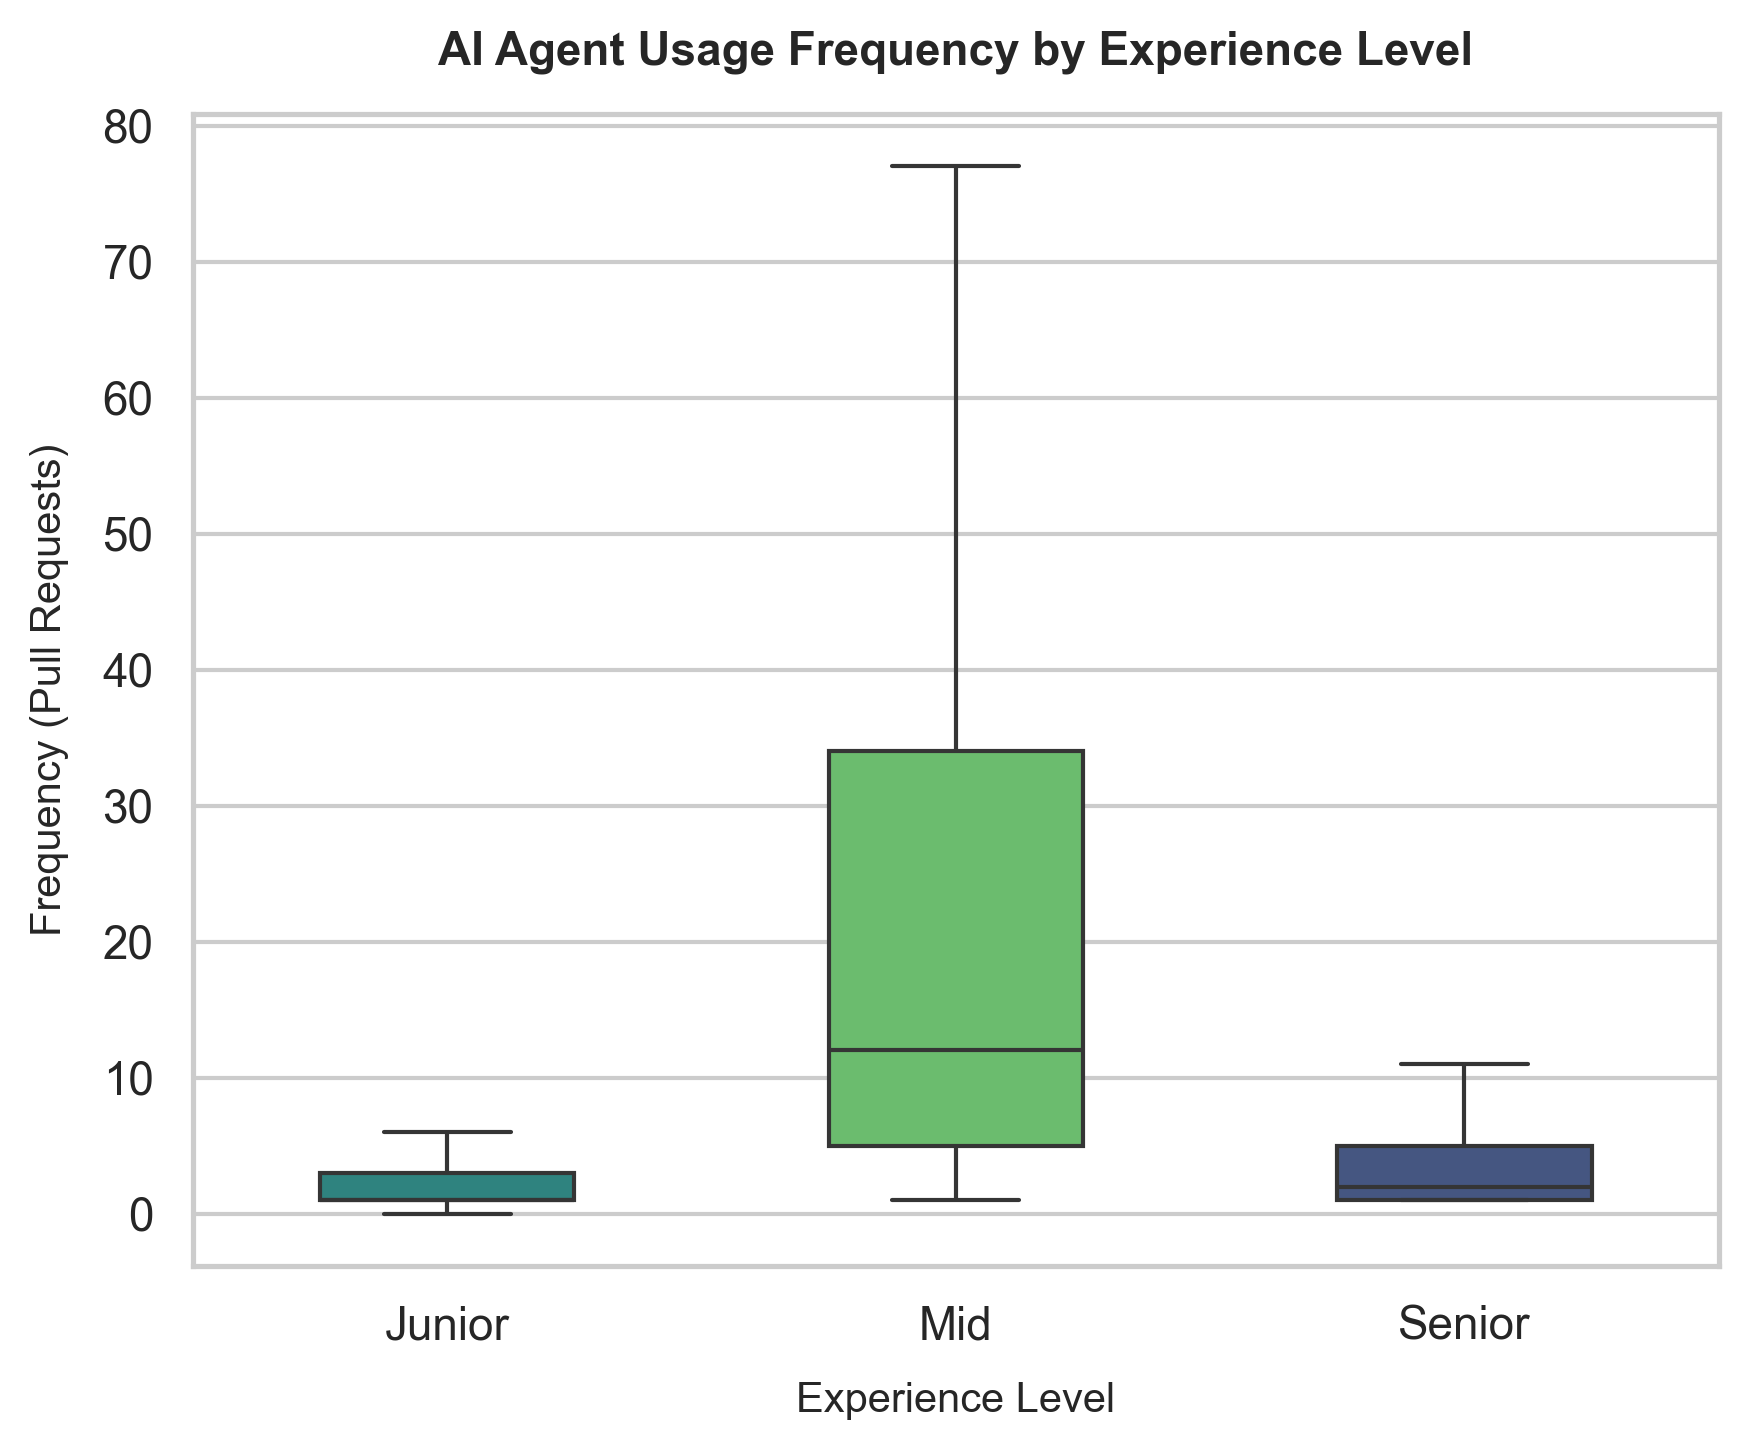
\includegraphics[width=0.85\linewidth]{box_plot.png}
    \label{fig:box_plot-exp1}
\end{figure}

\subsection{Does human experience translate into a higher acceptance rate of agent-generated code?}


The analysis performed shows that a developer's level of experience affects the acceptance rate of code generated by AI agents. The Kruskal-Wallis test confirmed the existence of significant differences between the studied groups. A detailed analysis using post-hoc tests (Mann-Whitney U with Bonferroni correction) reveals the following relationships:

\begin{itemize}
    \item Developers at the \textbf{Mid} level achieve the highest average code acceptance rate as well as the highest median. 
    
    \item Code generated by \textbf{Seniors} shows a lower median acceptance rate among the other groups, but the tests did not show significant differences between the remaining groups ($p=0.43$ for \textbf{Juniors} and $p = 1.00$ for \textbf{Mids})
\end{itemize}

Based on the data, it can be concluded that human experience does not automatically translate into a higher code acceptance rate. Developers at the \textbf{Mid} level show the greatest effectiveness in accepting AI agent proposals.

\begin{figure}[H]
    \centering
    
\includegraphics[width=1\linewidth]{second_experiment_box_plot.png}
    \label{fig:boxplot-exp2}
\end{figure}
 \begin{figure}[H]
     \centering
     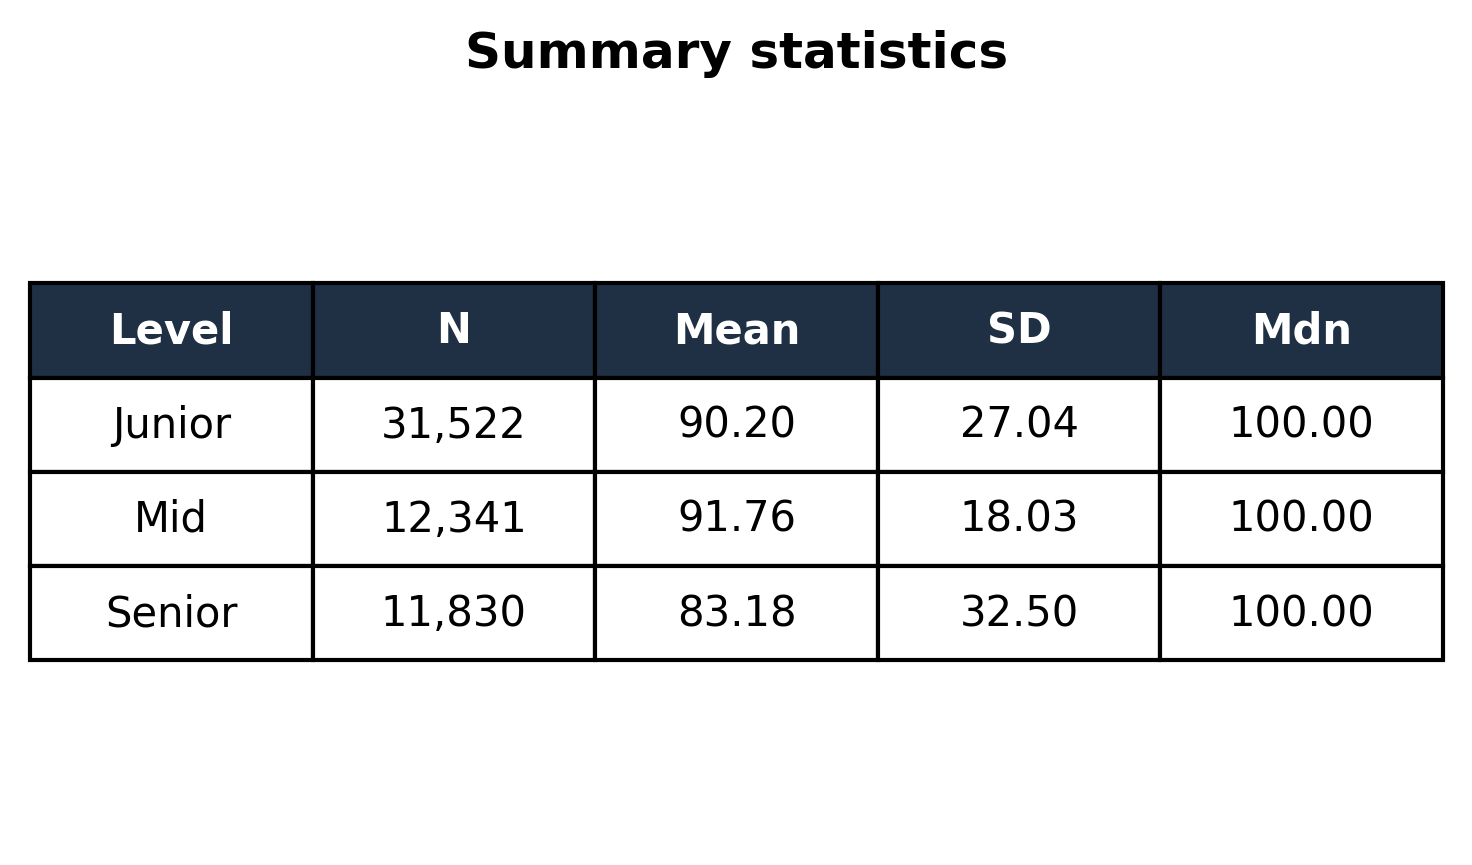
\includegraphics[width=1\linewidth]{second_boxplot.png}
     \label{fig:summary-exp2}
 \end{figure}


\subsection{Do changes introduced by the junior group using AI require more corrections (measured by the number of comments) from the project maintainer?}
The analysis was based on counting comments left by maintainers within \textit{pull requests}. In cases where the author of a \textit{pull request} turned out to be a bot, the associated \textit{issue} was checked, and its creator was treated as the actual author of the changes.

To verify this hypothesis, the \textbf{Kruskal-Wallis} test was used (robust to a large number of zero values in the data). The test confirmed the existence of statistical differences between all groups. Analysis using Mann-Whitney tests with Bonferroni correction showed that the differences are significant at every level of comparison:
\begin{itemize}
    \item \textbf{Junior} vs \textbf{Mid}: $p < 0.001$ 
    \item \textbf{Junior} vs \textbf{Senior}: $p < 0.001$ 
    \item \textbf{Mid} vs \textbf{Senior} $p < 0.001$
\end{itemize}

Code generated or supported by AI in the case of Juniors produced the lowest average number of comments. The highest rate was recorded in the \textbf{Mid} group. This result is somewhat surprising in the context of the hypothesis posed, and may result from the fact that Juniors create relatively simpler \textit{pull requests}, while Mids undertake more complex changes that generate more remarks from maintainers - not necessarily due to lower code quality.

\begin{figure}[H]
    \centering
    
\includegraphics[width=1\linewidth]{third_experiment_table.png}
    \label{fig:table-exp3}
\end{figure}

\begin{figure}[H]
    \centering
    
\includegraphics[width=1\linewidth]{third_experiment.png}
    \label{fig:boxplot-exp3}
\end{figure}
